En esta parte de la investigación se presentan algunos antecedentes relacionados a la detección y diagnóstico de nódulos en distintos órganos y a través de diversas metodologías. Estos ayudarán a entender el enfoque y obtener bases para un correcto desarrollo del proyecto en cuestión.

\cite{pr_moreira2021deteclung} presenta una investigación relacionada a la elaboración de un sistema CAD (Computer-aided Detection) para la detección y segmentación de nódulos presentes en los pulmones.

Para realizar esta investigación, se tuvo en consideración la realidad que se atraviesa a nivel mundial sobre el cáncer de pulmón, y como este afecta a las personas sin importan su género, convirtiéndolo uno de los tipos de cáncer más mortales según la investigación mencionada. 

La presencia de nuevas formas de detectarlo como el uso de tomografías computarizadas tuvo un gran impacto para la detección temprana de los nódulos en estos órganos, ya que estos pueden significar un futuro desarrollo de cáncer. Sin embargo, realizar un análisis de este tipo de imágenes médicos no era nada trivial debido al complejo proceso de análisis con estas tecnologías. Ante esto, el Deep Learning apareció con una herramienta eficaz para ayudar a los médicos en el análisis de estas imágenes; sin embargo, pese a sus grandes ventajas, su aplicabilidad es muy limitada. Por tal motivo, esta tesis incluye modernos enfoques y técnicas para una detección automática de nódulos pulmonares.

De forma general, el algoritmo presentado en esta investigación consiste en dos bloques. El primero de estos se encarga de la detección de nódulo a través de técnicas de detección de objetos, mientras que el segundo se encarga de la segmentación de este. Los resultados obtenidos fueron del 79\% en recall; sin embargo, esto no fue suficiente para poder considerar al modelo como robusto, por ello, posteriormente, se utilizaron técnicas innovadoras en colaboración expertos en el área. Las anotaciones de los especialistas, junto con los resultados del sistema, mejoraron el desempeño general de la detección.

Para aumentar aún más las capacidades del sistema, se desarrolló en la parte final de la investigación un modelo de Deep Learning para la detección automática y la segmentación de nódulos pulmonares a través de imágenes tomográficas. Este también consistió en dos bloques, uno encargado de la segmentación automática y otro que corrige el anterior en base a dos puntos en los límites del nódulo. El modelo consiguió demostrar su capacidad para corregir la segmentación de nódulos pequeños, además de segmentar los nódulos no sólidos, los cuales presentaban un reto para el sistema.

\cite{pr_felgueiras20193dlungnod} reafirman la importancia de construir este tipo de sistemas mencionando al cáncer de pulmón como el principal tipo de cáncer en causar muertes en todo el mundo.

El sistema desarrollado en esta investigación fue basado también en el diagnóstico a través de imágenes tomográficas que comúnmente es realizado por un médico experto; sin embargo, se menciona que este análisis siempre está sujeto a errores ya que existe mucha subjetividad en este tipo de diagnóstico, lo que conlleva muchas veces errores de detección. Además de la existencia de la tendencia al rechazo hacia esto tipo de sistemas CADx (Computer-aided Diagnosis) por parte de los médicos, esto debido a la fata de comprensión del cómo se realiza este tipo de diagnóstico.

Para afrontar esta desconfianza a este tipo de sistemas, se menciona la existencia del Deep hierarchical semantic convolutional neural network (HSCNN) que añadía a la capacidad de predecir si un nódulo era maligno o benigno, la función de otorgar evidencia visual del diagnóstico a través de la predicción de las características del nódulo. Sin embargo, el conjunto de datos usado en esta investigación difería de las evaluaciones de los propios médicos. Por tal motivo, en la presente investigación se puso como un objetivo probar si la disminución de esta varianza en los datos podría mejorar los resultados del modelo HSCNN.

A través de un análisis de los datos, se logró mejorar la descripción de características. Este nuevo conjunto de datos fue revisado por especialista para comprobar su validez antes de ser ingresado al modelo HSCNN para predecir si un nódulo era maligno o benigno. Este proceso se hizo a través de un k-folds igual a 4 junto con cross-validation.

Los resultados fueron comparados con el modelo inicial, y se obtuvo que el nuevo HSCNN era mejor solo cuando se trataba de predecir si un nódulo era maligno. Las métricas del nuevo modelo fueron de 0.78 en accuracy, el AUC de la curva ROC es de 0.74, una sensibilidad 0.83 y una especificidad de 0.89, frente a las métricas de modelo original que obtuvo un accuracy de 0.84, un AUC de la curva ROC de 0.86, sensibilidad de 0.71 y una especificidad de 0.89. Esto significó que el modelo se equivocaba más cuando los nódulos a analizar eran pequeños. En general, los resultados distaron de los propios del modelo inicial, esto es debido a la reducción considerable de imágenes del conjunto de datos original. 

\cite{pr_supanta2021desalgdetec} menciona la incidencia de cáncer de pulmón en el Perú en el periodo 2010-2012 con un gran número de 3 121 casos diagnosticados, convirtiéndolo en el tercer tipo de cáncer más común en el país, y ocupa el segundo lugar en mortalidad con un número de 2 591 de muertes en el mismo periodo, esto debido al tardío diagnóstico de este mal. Por este motivo, es obvia la necesidad de realizar un examen de detección temprana donde es posible un tratamiento y, posteriormente, una posible cura a esta enfermedad. 

La investigación presenta una forma de realizar detección de nódulos pulmonares a través de imágenes radiográficas digitales que comúnmente presentan problemas como baja claridad y resaltado de las características, por ende, generan dificultades para realizar un correcto análisis de este tipo de imágenes. Las técnicas usadas son corrección gamma, análisis de proyecciones, erosión, filtros geométricos, dilatación, filtro de convergencia y la umbralización por el método Otsu, esto aplicado a un conjunto de datos de 50 radiografías de tórax.

Los resultamos muestran una sensibilidad del 0.91, especificidad de 0.96 y precisión de 0.94. 

Otra investigación relacionada a detectar alguna enfermedad a través de técnicas de Deep Learning y visión por computadora es la presentada por \cite{pr_monroy2021disvc} donde toma a la enfermedad de Parkinson como mal a detectar, y esto a través del análisis de la escritura de una persona. Para tal objetivo, en la investigación se desarrolló un modelo de visión computacional para el prediagnóstico de esta enfermedad.

La metodología empieza con la adquisición y preprocesamiento de los datos, para posteriormente usar técnicas de extracción de características como SIFT, SURF, ORB y HOG. Estos serán ingresados a un modelo de Machine Learning (SVM, RF, KNN) que finalmente realizará una clasificación. Además, se usaron diferente arquitectura de redes neuronales convolucionales como Inception, VGG16, VGG19, LeNet y ResNet50.

Los resultados finales fueron un 0.99 en accuracy, 0.99 en precisión, 0.99 en recall, 0.98 en F1-score y AUC.

\cite{pr_kang2022thysegclass} muestran la frecuencia de diagnóstico de nódulos tiroideos, esto en el rango de 19\% y 68\% de casos clínicos. El cáncer de tiroides es el número 9 en incidencia, mientras que es el número 6 en mortalidad, esto a nivel mundial según datos del 2018.

Se menciona que es importante tener métodos menos invasivos para determinar el cáncer de tiroides, teniendo en cuenta además que es necesario la detección a tiempo, pues esto aumenta la probabilidad de ser curado. El análisis de imágenes de ultrasonido es una buena opción a el análisis de, por ejemplo, cirugías. Sin embargo, este diagnóstico depende mucho de la experiencia del médico especialista, lo cual vuelve a este tipo de análisis muy subjetivo.

La segmentación y clasificación son herramientas claves dentro de un sistema de diagnóstico asistido, siendo ambos muy relacionados entre sí, pues comparten ciertas características de las imágenes (bordes de las imágenes pueden ser usados para la clasificación y segmentación). Afrontar ambas tareas al mismo tiempo en un solo modelo podría ser más robusto.

La red MTL propuesta en uno de los antecedentes es similar a una red de segmentación multiclases que genera como salida mapa de segmentación y predicciones categóricas.

La investigación presentada en este antecedente se centra también en una red MTL que también realizará procesos de segmentación y clasificación.

La metodología empieza con la data. Esta fue recolectada del West China Hospital. Se tuvieron 4 493 imágenes de ultrasonido, cada uno de un paciente. En específico, 2 576 imágenes pertenecen a nódulos benignos, mientras que 1 917 son malignos. Las anotaciones fueron verificadas por especialistas.

Para la evaluación de la clasificación se usó el accuracy, f1-score, ROC, área bajo la curva ROC (AUC). En el caso de la segmentación, se usó Dice coefficient y Intersection of Union (IoU).

Además, se definieron 3 medidas para cuantificar la inconsistencia al nivel de las tareas. El primero de estos evalúa a la clasificación, el segundo por la tarea de segmentación de segunda clase, y el tercero es para la segmentación de tercera clase.

El modelo construido en esta investigación se basó en MSL (Multi Stage Learning) y MTL (Multi Task Learning). Se diseño una red MS-MTL. Además, se determinó diferentes tipos de consistencia de tareas: intra e inter task consistency.

Los resultados fueron extraídos de 3 modelos CIsNet, MS-MTL y MS-MTL con intra e inter task consistency. La medida AUC obtenida para cada modelo es 0.9277, 0.9523 y 0.9608, respectivamente. Además, se determinó que el intra task cosistency y el MSL aumenta el desempeño de la segmentación. El caso de inter task consistency con MTL mejora el desempeño de las tareas de clasificación y segmentación. Con la combinación de ambas tareas de consistencias también se demuestra su efectividad.

El método usado en esta investigación se muestra a continuación.

\begin{figure}[H]
	\begin{center}
		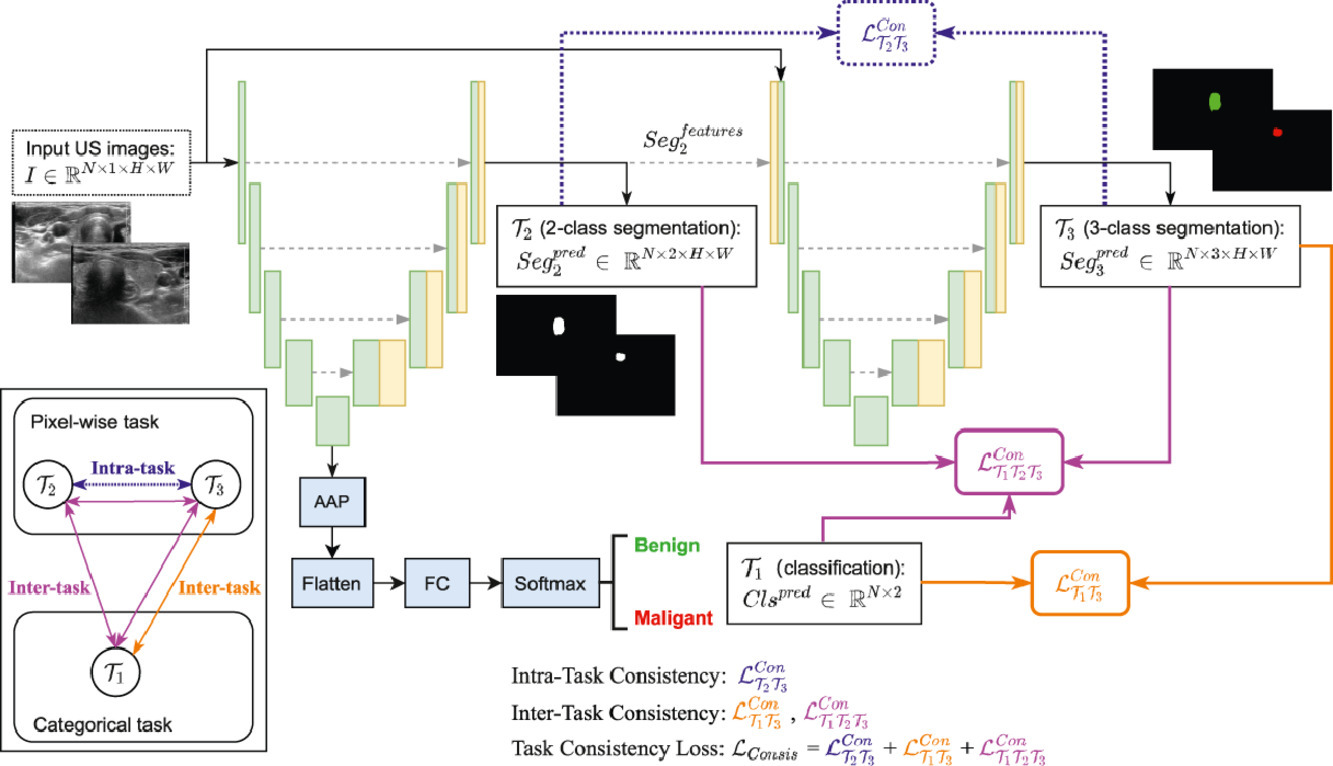
\includegraphics[width=1.00\textwidth]{2/figures/antecedente_4.jpg}
		\caption[Representación del método desarrollado]{Representación del método desarrollado. \\
		Fuente: \cite{pr_kang2022thysegclass}. \textit{Thyroid nodule segmentation and classification in ultrasound images through intra- and inter-task consistent learning}.}
		\label{2:fig101}
	\end{center}
\end{figure}


\cite{pr_sun2023classthynvit} presenta el problema de diagnosticar nódulos tiroideos nivel 3 debido a pocas características representativas que diferencien a los nódulos benignos de nivel 3 con los nódulos malignos, esto conlleva a obtener bajas precisiones en el diagnóstico. Ante esto, en el artículo se presenta un modelo clasificador de nódulos tiroideos con ViT (Vision-Transformer-based) y el contrast learning. Estas técnicas ayudaron a minimizar la distancia de características en nódulos de una misma clase, lo cual mejora la capacidad predictiva del modelo. Finalmente, en la fase de testeo del modelo se logró un accuracy de 0.869, mientras que las demás métricas indican la superioridad frente a otros modelos clásicos de Deep Learning que también son usados para clasificar.

En la siguien figura se presenta la arquitectura de Vison Transformer desarrollada.

\begin{figure}[H]
	\begin{center}
		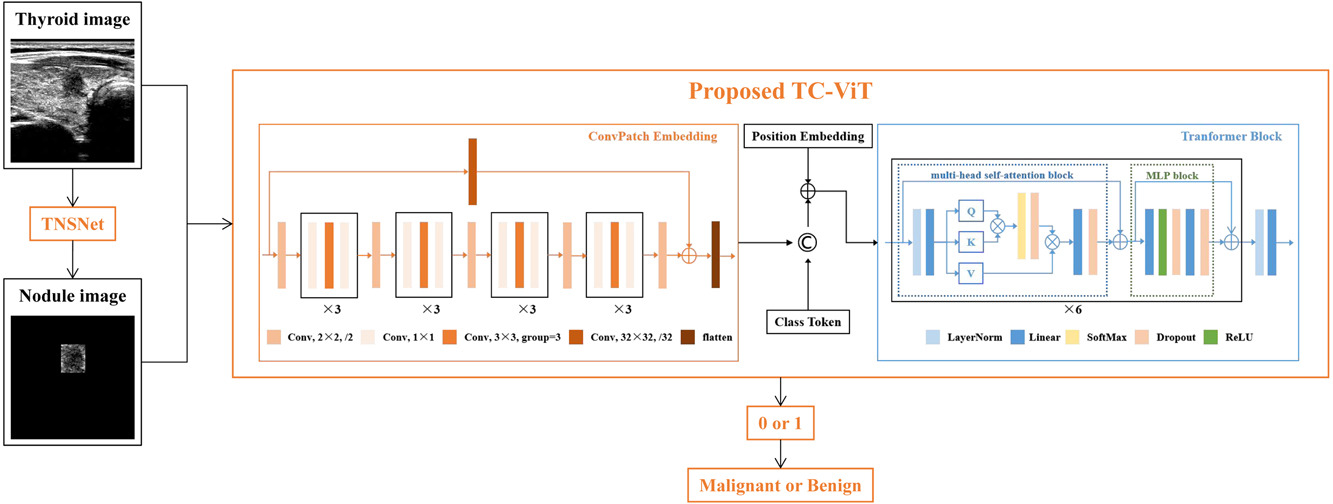
\includegraphics[width=1.00\textwidth]{2/figures/antecedente_5.jpg}
		\caption[Arquitectura de modelo TC-ViT]{Arquitectura de modelo TC-ViT. \\
		Fuente: \cite{pr_sun2023classthynvit}. \textit{Classification for thyroid nodule using ViT with contrastive learning in ultrasound images}.}
		\label{2:fig102}
	\end{center}
\end{figure}


\cite{pr_zhang2023madlap} presenta el nivel de importancia de poseer una buena base de datos etiquetada correctamente para lograr entrenar un buen modelo de Machine Learning. En este artículo se desarrolla y presenta a la herramienta Multistep Automated Data Labelling Procedure (MADLaP) que facilita y automatiza el proceso de etiquetado de datos relacionados a nódulos tiroideos. Este incluye el procesamiento de leguaje natural basado en reglas, el Deep Learning para segmentación de imágenes y el reconocimiento óptico de caracteres. MADLaP fue desarrollado en la fase de entrenamiento con datos de 378 pacientes, mientras que en la fase de prueba se usaron datos de 93. Este obtuvo finalmente un accuracy de 0.83.

\cite{pr_deng2022autclass} ponen al cáncer de tiroides como el que más ha prevalecido en las últimas 3 décadas. Existen diversos sistemas que ayudan a la detección de los nódulos en esta glándula; sin embargo, muchos de estos solo se limitan a determinar si un nódulo es maligno o benigno, y no muestran el porqué de la toma de esa decisión por parte del sistema, lo cual genera desconfianza entre los especialistas al momento de usarlos. Para afrontar esto, se desarrolla primeramente una estratificación de riesgo basada en el léxico estandarizado ACR TI-RADS. Posteriormente, se realiza la clasificación entre benigno y maligno. De formar general, el método realizará una caracterización del nódulo basado en ACR TI-RADS para detectar su nivel de riesgo y la clase al que pertenece (benigno o maligno). Los resultados muestran en la evaluación un accuracy de 0.9355, un sensitivity de 0.9386 y una specificity de 0.9314. 

Se realizó la notación de las imágenes de nódulos con los indicadores del diccionario de ACR TI-RADS. Para afrontar el desbalanceo de la data, se realizó un proceso de mejora de la data creando imágenes a través de giros, recortes y mezclas. Se extrajeron las áreas de interés de las imágenes a través de una red en cascada. Se quitaron las anotaciones manuales en las imágenes (limpieza de imagen). Una vez concluido con el procesamiento de las imágenes, se realizó la construcción y ejecución del modelo de Deep Learning Multi-Task Learning (MLT). Finalmente, el modelo obtenido fue comparado con otros a través de los siguientes indicadores: accuracy, sensitivity, specificity y el área bajo la curva. 

\cite{pr_wang2020autodiag} mencionan que los nódulos tiroideos son uno de los primeros síntomas que podrían conllevar a un cáncer en la tiroides. Este tipo de cáncer es uno de los que tiene mayor incidencia y que esta tendencia ha ido en crecimiento durando los últimos 30 años.

Además, se menciona que, para ayudar a esta detección, se han propuesto anteriormente varios sistemas de diagnóstico asistido; sin embargo, estos solo realizan dicho proceso a través de solo una imagen de ultrasonido en vez de usar todas aquellas que se obtienen de un examen. Por esto, en este artículo, se desarrolla un modelo de Deep Learning para el diagnóstico de tiroides a través de varias imágenes de ultrasonido. Esto a través de una integración de todas las características de las imágenes realizadas en un examen. 

La base de datos usada fue construida, y se obtuvieron resultados perfectamente comparables con los resultados de los antecedentes revisados en este artículo.

La metodología consistía en la construcción de tres redes distintas: feature extraction network, attenntion-based feature aggregation network, classification network. Estas tres redes juntas forman el modelo objetivo desarrollado en este artículo.

En general, la metodología consistía en, primero, la construcción del conjunto de datos que se conforma de imágenes de ultrasonido procedentes de un hospital. Se recolectaron cerca de 7 800 imágenes de 1 046 exámenes de entre los años 2015 y 2018. En segundos lugar, se realizó el etiquetado de los datos. Estas anotaciones se realizaron de acuerdo con los exámenes en general, y no a cada una de las imágenes que la conforman. Luego, se realizó la separación de la data en entrenamiento, prueba y validación. En la parte final de experimentación, se realizó un preprocesamiento con data augmentation y se definió 100 épocas para la fase de entrenamiento. El modelo ganador de la fase de validación fue probado con la data de prueba. Las métricas usadas para la evaluación fueron el accuracy, sensitivity (true positive rate) y el área bajo la curva (AUC ROC).

La siguiente figura muestra la arquitectura propuesta en esta investigación.

\begin{figure}[H]
	\begin{center}
		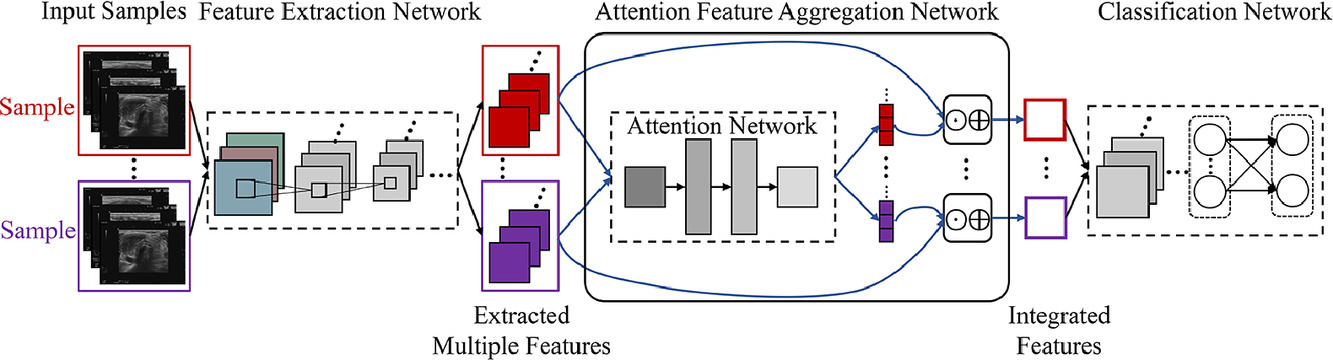
\includegraphics[width=1.00\textwidth]{2/figures/antecedente_8.jpg}
		\caption[Arquitecura de la red desarrollada]{Arquitecura de la red desarrollada. \\
		Fuente: \cite{pr_sun2023classthynvit}. \textit{Automatic diagnosis for thyroid nodules in ultrasound images by deep neural networks}.}
		\label{2:fig103}
	\end{center}
\end{figure}


\cite{pr_sun2022tnsnet} mencionan que, en el sistema endocrino, un problema muy común son los nódulos tiroideos. Normalmente estos pueden ser sólidos o de otras variadas texturas. La incidencia de esta enfermedad se ha ido incrementando a través de los años. Comúnmente se usan las imágenes de ultrasonido para detectar estos nódulos, esto lo hacen en tiempo real, tiene bajo costo y no es invasivo, por cual es una buena opción. Estas imágenes pueden otorgar información valiosa de los nódulos como los márgenes, ecogenicidad, calcificación, composición, etc. Además, existe el Thyroid Image Reporting y el sistema de datos TI-RADS pueden cuantificar las características otorgadas por las imágenes de ultrasonido y evaluar si es benigno o maligno. Sin embargo, estas imágenes pueden traer problemas como bajo contraste y ruido de moteado, lo cual genera retos para extraer sus características. Este problema puede superarse a través de una correcta segmentación de los nódulos tiroideos. Así, la segmentación es un paso importante para realizar diagnóstico correcto. Esto puede ser aplicado a la evaluación automática en TI-RADS para facilitar la clasificación de los nódulos. Se añadió un shape-supervised path para mejorar la identificación de la forma, y así lograr una mejor segmentación.

La data que usaron se obtuvo de diversos escáneres disponibles comercialmente, juntando 3 786 imágenes de ultrasonido de nódulos tiroideos. Posteriormente, se realiza un preprocesamiento para estandarizar la data. Se realizó un proceso de limpieza de las imágenes para quitar los datos privados de los pacientes, y borrar imágenes erróneas. Se propuso TNSNet para asegurar una mejor detección y segmentación. Este modelo es un dual-path network que contiene dos partes region path y shape path. Ambos caminos se enfocan en las características de bordes y texturas (cada uno de estos para cada camino).

Se diseñó un dual-path loss function para el entramiento de ambos caminos del modelo. Para el camino de región, se usó el binary cross-entropy loss y el generalized Dice loss, ambos para entrenar la región de segmentación de los nódulos tiroideos. En el caso del segundo camino (camino de la forma) se combinó el Hausdoff distance loss y un modificado active contour loss. Esto fue construido para el entrenamiento del contorno de segmentación.

Las métricas usadas para evaluar la segmentación del modelo son Dice simialrity coefficient (DSC), sensitivity, specificity y el accuracy.

Los resultados muestran que en el caso de los nódulos benignos todos los modelos (el construido en el artículo y los de referencia) logran buenos resultados, esto debido a la buena calidad de las imágenes. En el caso de los nódulos malignos, el modelo TNSNet superó por completo a los otros modelos de referencia. Hubo otros experimentos, en los cuales, el modelo presentado en este artículo, de manera general, obtuvo mejores resultados.

La investigación realizada por \cite{pr_yang2023novelViTscc} se centra en la problemática del cáncer de piel, específicamente en el grave problema de los melanomas y la alta necesidad de una detección temprana para mejorar las posibilidades de supervivencia de los pacientes con este mal.

Además, se menciona que aunque la técnica más usada para la detección de melanomas es la dermatoscopia, su precisión es muy variada dependiendo el tipo de cáncer de piel con el que se está tratando. En este contexto, las técnicas de Deep Learning han demostrado ser un herramienta capaz de mejorar la precisión en las tareas relacionadas a clasificar el cáncer de piel, incluso superando al desempeño de los propios dermatólogos.

A pesar de estos logros del desarrollo de Deep Learning en esta área, se menciona que aún hay dificultad para la clasificación de algunos tipos de cáncer de piel como el melanoma. Por este motivo se propone una nueva arquitectura de red basada en los transformadores con el objetivo de mejorar la capacidad de los algoritmos de clasificación de cáncer de piel.

La metodología seguida por los autores inicia con la preparación de los datos. En este caso se usó el conjunto de datos HAM10000 que consta de 7 clases distintas de cáncer de piel. Las imágenes tuvieron que ser redimensionadas para los 4 distintos modelos a entrenar: Inception ResNet con Soft Attention (IRv2 + SA), ResNet50 con Soft Attention (ResNet50 + SA), ViTfSCD-Large y ViTfSCD-Base. Los parámetros de estos dos últimos modelos se muestran en la siguiente figura.

Además, se aplicó a las imágenes una limpieza, eliminando los duplicados. También pasó por un proceso de balanceo de las clases donde se intentó igualar la cantidad de imágenes en cada una de estas. Se realizó el proceso de aumento de datos a través de modificaciones en las imágenes como alterar la saturación de forma aleatoria, cambiar el contraste y el brillo. Finalmente, se definió los porcentajes de división para el conjunto de datos, siendo 85\% para el entrenamiento y 15\% para la prueba. 

Para la evaluación de los modelos se utilizaron las métricas de accuracy, precision, recall (sensitivity), specificity y F1 score. Los resultados de evaluar su capacidad de clasificación de los 4 modelos se muestran a continuación.

\begin{figure}[H]
	\begin{center}
		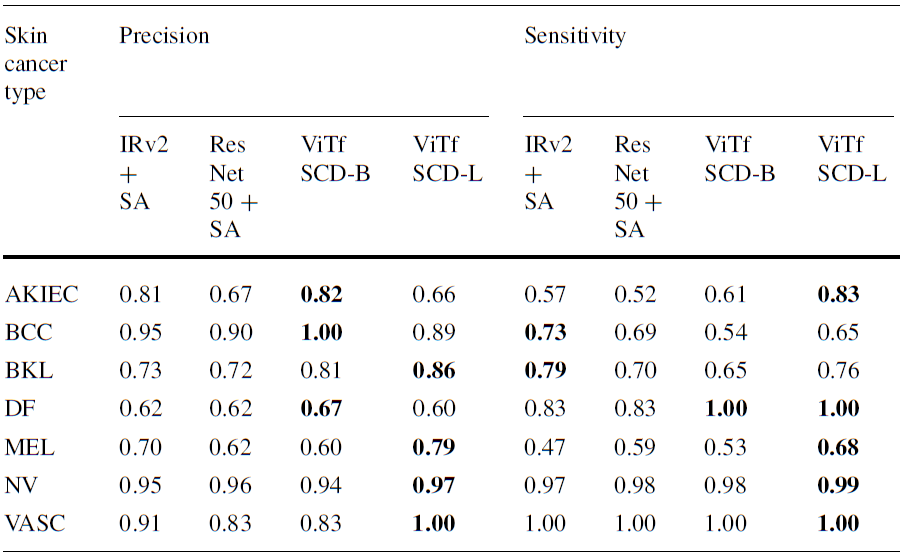
\includegraphics[width=1.00\textwidth]{2/figures/vitpaper1_part1.png}
		\caption[Comparación de resultados de los modelos (precision y sensitivity)]{Comparación de resultados de los modelos (precision y sensitivity). \\
		Fuente: \cite{pr_yang2023novelViTscc}. \textit{A Novel Vision Transformer Model for Skin Cancer Classification}.}
		\label{2:fig104}
	\end{center}
\end{figure}

\begin{figure}[H]
	\begin{center}
		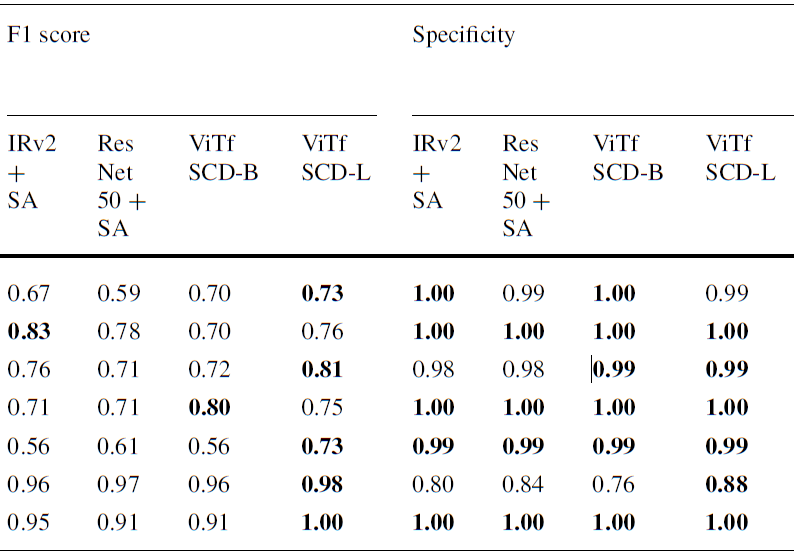
\includegraphics[width=1.00\textwidth]{2/figures/vitpaper1_part2.png}
		\caption[Comparación de resultados de los modelos (f1-socre y specificity)]{Comparación de resultados de los modelos (f1-socre y specificity). \\
		Fuente: \cite{pr_yang2023novelViTscc}. \textit{A Novel Vision Transformer Model for Skin Cancer Classification}.}
		\label{2:fig105}
	\end{center}
\end{figure}

De los resultados, se observó que el modelo ViTfSCD-Large obtuvo el más alto precision, recall, y F1 scores. Además, el mismo modelo obtuvo un accuracy de 94.1\%, siendo el valor más alto, mientras que el modelo ViTfSCD-Base obtuvo 91.4\%.

Finalmente, se realizó una comparación de los modelos a través de su accuracy. En esta última sección, se comparó con otros modelos del estado de arte desarrollados con el conjunto de datos HAM10000. El primero de estos, implementado en 2020 y denominado Efficient-Net logró un accuracy de 92.6\%. También, en el año 2021, se desarrolló un método semi supervisado para la clasificación de imágenes médicas que obtuvo un accuracy de 92.5\%. 

Para esta comparación final, también se consideraron los resultados originales de los modelos IRv2, IRv2 + SA, ResNet50 y ResNet50 + SA junto con los resultados obtenidos en esta investigación. Además, también se realizaron experimentos con los modelos ViT originales (ViT-Base 16 y ViT-Large 16). Los resultados finales muestran que los modelos ViTfSCD-Base y ViTSCD-Large son superiores a sus versiones originales.

\begin{figure}[H]
	\begin{center}
		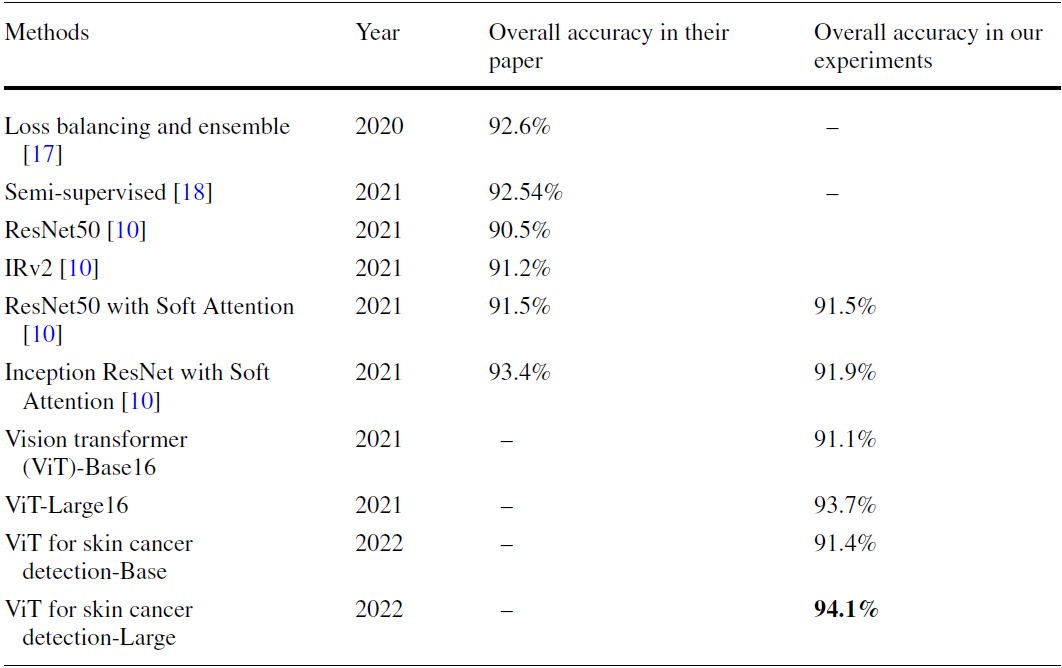
\includegraphics[width=0.90\textwidth]{2/figures/vitpaper1_part3.png}
		\caption[Comparación de resultados según accuracy con el conjunto de datos HAM10000]{Comparación de resultados según accuracy con el conjunto de datos HAM10000. \\
		Fuente: \cite{pr_yang2023novelViTscc}. \textit{A Novel Vision Transformer Model for Skin Cancer Classification}.}
		\label{2:fig106}
	\end{center}
\end{figure}

También se realizaron experimentos con el conjunto de datos DERMOFIT que consta de imágenes de lesiones clínicas de la piel divididas en 10 clases distintas. Los resultados originales con este conjunto de datos muestran que el modelo ResNet50 tuvo mejor desempeño que el modelo de árbol de decisión y KNN. 

Los nuevos experimentos con este conjunto de datos se llevaron a cabo con los modelos ResNet50, IRv2 y ViTfSCD-Base. Los siguientes resultados muestran el desempeño superior del modelo ViTfSCD frente a los demás.

\begin{figure}[H]
	\begin{center}
		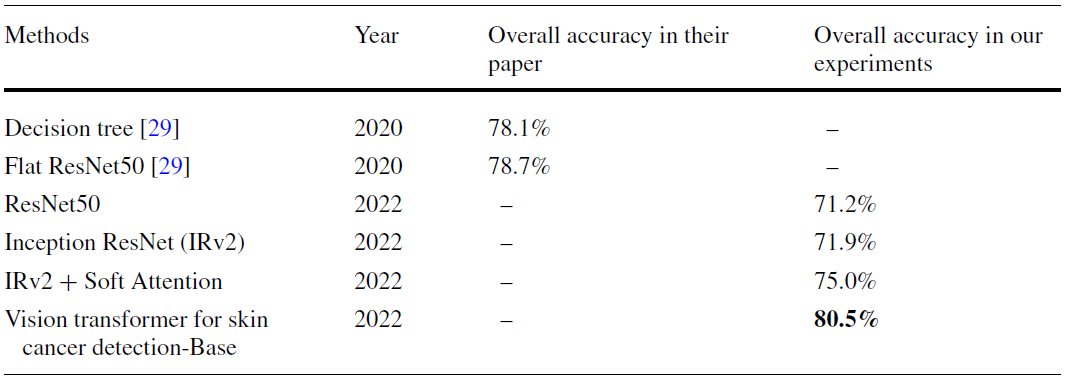
\includegraphics[width=1.00\textwidth]{2/figures/vitpaper1_part4.png}
		\caption[Comparación de resultados según accuracy con el conjunto de datos DERMOFIT]{Comparación de resultados según accuracy con el conjunto de datos DERMOFIT. \\
		Fuente: \cite{pr_yang2023novelViTscc}. \textit{A Novel Vision Transformer Model for Skin Cancer Classification}.}
		\label{2:fig107}
	\end{center}
\end{figure}
